\documentclass{standalone}
\usepackage[T1]{fontenc}
\usepackage[utf8]{inputenc}
\usepackage[usenames,dvipsnames]{xcolor}
\usepackage{tikz}
\usetikzlibrary{plotmarks}
\usetikzlibrary{shapes,snakes,arrows}
\begin{document}
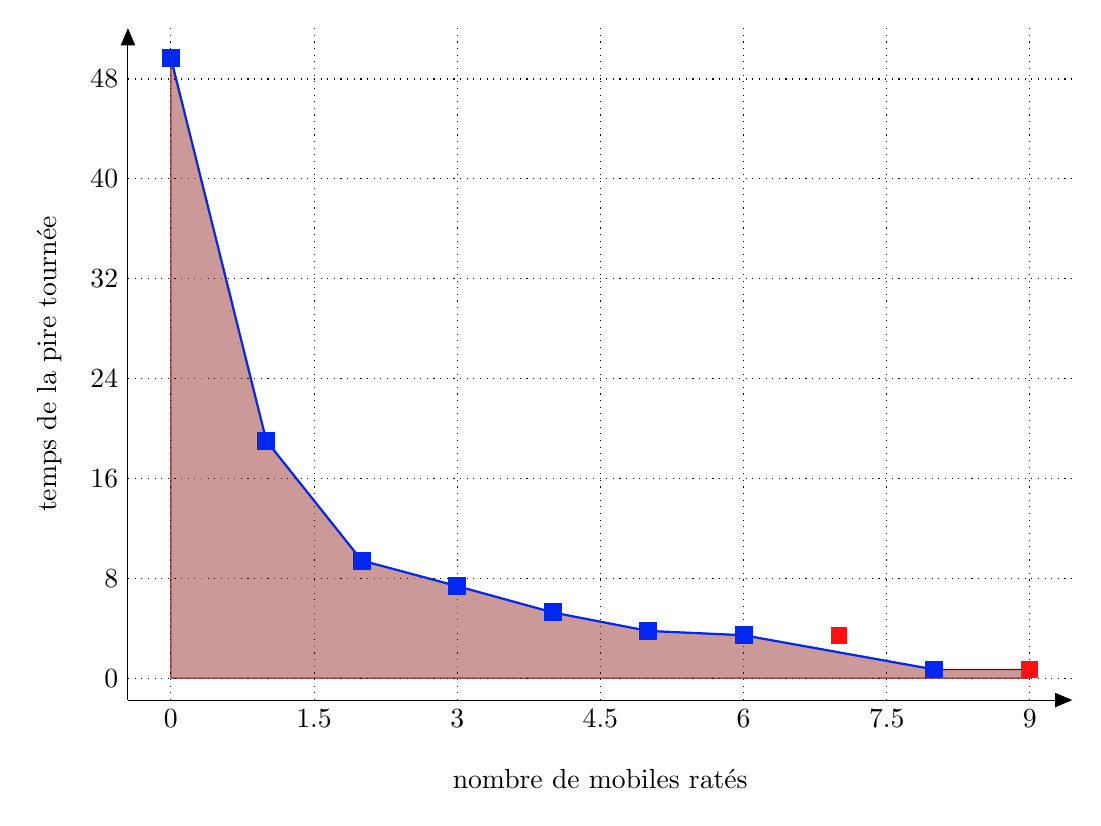
\begin{tikzpicture}[xscale=1.21212,yscale=0.1585229]
\draw[xstep=1.5,ystep=8,thin,dotted,color=Black] (-0.45,-1.75657) grid (9.44448,52.0675);
\begin{scope}
  \clip (-0.45,-1.75657) rectangle (9.44448,52.0675);
  \definecolor{hvColor}{RGB}{128,0,0}
  \draw[color=hvColor, fill=hvColor, fill opacity=0.4] (0,0.692884) -- (0,49.682) -- (1,19.0169) -- (2,9.42242) -- (3,7.37304) -- (4,5.26681) -- (5,3.78305) -- (6,3.43859) -- (8,0.692884) -| (9,0.692884) |- (0,0) -- cycle;
  \definecolor{pLineColor}{RGB}{128,0,0}
  \definecolor{pPointColor}{RGB}{0,40,240}
  \draw[thick,color=pPointColor] (0,49.682) node[draw,color=pPointColor,fill=pPointColor, inner sep = 0pt, minimum size=2mm] {} -- (1,19.0169) node[draw,color=pPointColor,fill=pPointColor, inner sep = 0pt, minimum size=2mm] {} -- (2,9.42242) node[draw,color=pPointColor,fill=pPointColor, inner sep = 0pt, minimum size=2mm] {} -- (3,7.37304) node[draw,color=pPointColor,fill=pPointColor, inner sep = 0pt, minimum size=2mm] {} -- (4,5.26681) node[draw,color=pPointColor,fill=pPointColor, inner sep = 0pt, minimum size=2mm] {} -- (5,3.78305) node[draw,color=pPointColor,fill=pPointColor, inner sep = 0pt, minimum size=2mm] {} -- (6,3.43859) node[draw,color=pPointColor,fill=pPointColor, inner sep = 0pt, minimum size=2mm] {} -- (8,0.692884) node[draw,color=pPointColor,fill=pPointColor, inner sep = 0pt, minimum size=2mm] {};
  \definecolor{pLineColor}{RGB}{255,16,16}
  \definecolor{pPointColor}{RGB}{255,16,16}
  \node[draw,color=pPointColor,fill=pPointColor, inner sep = 0pt, minimum size=2mm] at (7,3.43859) {};
  \node[draw,color=pPointColor,fill=pPointColor, inner sep = 0pt, minimum size=2mm] at (9,0.692884) {};
\end{scope}
\draw[->,>=triangle 45] (-0.45,-1.75657) -- coordinate (x axis mid) (9.44448,-1.75657);
\node[below=1cm,anchor=center] at (x axis mid) {nombre de mobiles ratés};
\foreach \x in {0,1.5,3,4.5,6,7.5,9}
  \draw (\x,-1.75657) -- (\x,-1.75657) node[anchor=north] {\x};
\draw[->,>=triangle 45] (-0.45,-1.75657) -- coordinate (y axis mid) (-0.45,52.0675);
\node[left=1cm,rotate=90,anchor=center] at (y axis mid) {temps de la pire tournée};
\foreach \y in {0,8,16,24,32,40,48}
  \draw (-0.45,\y) -- (-0.45,\y) node[anchor=east] {\y};
\end{tikzpicture}
\end{document}
